\chapter{Methods}
In this chapter the methods needed to create a parametric model and  a mapping between parametric models are introduced and explained. First off, the data gathering and preprocessing are outlined. Multiple variants of the parametric model are discussed. Different learning approaches for the mapping are reviewed. Lastly, a character editor is presented that is used to generate data for a parametric model.

\section{Data Acquisition and Preprocessing}
Optimally it would be necessary to have a large data set of images of women before and after breast enhancement surgery, where the patients pose topless. It is very unlikely though that such a database exists, due to the fact that having breast surgery is a very personal topic and people generally don't enjoy posing naked. Therefore the images used were downloaded from a website\footnote{https://my.crisalix.com/} that offered to simulate various plastic surgical procedures including breast enhancement. For each user a 3D model of their torse was displayed side by side with different enhancements varying in size. Each model was made up of a sequence of 24 images displaying the torse from different angles. This dataset fit the requirements nicely as images are available for \textit{before} and \textit{after}, except the \textit{after} is generated and based on their model. Additionally, each after image sequence had a short label, usually describing how much silicon was added, that was also saved for further evaluation. In total 2'937 examples were retrieved and preprocessed. This dataset included images from 748 subjects of which each one was comprised of one \textit{before} and at least one \textit{after} image sequence.\\

In a next step these image sequences needed to be transformed into point clouds. This was done using a general-purpose Structure-from-Motion (SfM) \cite{schoenberger2016sfm} and Multi-View Stereo (MVS) \cite{schoenberger2016mvs} pipeline called COLMAP. This generated point clouds spanning from 5'000 to 15'000 points. Some of the images needed to be discarded, due to the fact that SfM created a point cloud with less than 1'000 points or the point clouds had holes, such that certain areas had no points and were not defined at all. The remaining point clouds were cleaned using a C++ implementation by Biland \cite{Biland17} that removed white points around the point clouds.

The mapping required to have one set of point clouds of \textit{before} examples and the corresponding\footnote{Corresponding meaning, based on the same subject.} \textit{after} examples. Therefore the data was split into sets of \textit{before} and after point clouds. Additionally, to create a better mapping, only the \textit{after} examples that were labelled "350" were included. This resulted in 57 examples in the \textit{before} and 57 in the \textit{after} set. All of these point clouds were further processed in a MATLAB implementation by Biland \cite{Biland17} to generate mesh files.

\subsection{Alignment}
Eventhough the meshes were aligned in the MATLAB implementation by Biland \cite{Biland17} in a general fashion, each corresponding \textit{before} and \textit{after} should be pairwise aligned to avoid that the mapping also learns rotations. This was achieved by using an implementation of Horn's method \cite{horn1987closed}. Given two sets of vertices, Horn's method computes the translation, rotation and possibly scale change from one set to the other. As it is expected that for the same subject, only points defining the breasts should vary from before to after, only a subset of vertices should be used. The points used in the alignment can be seen in figure \ref{fig:alignment}.

\begin{figure}[h]
\centering
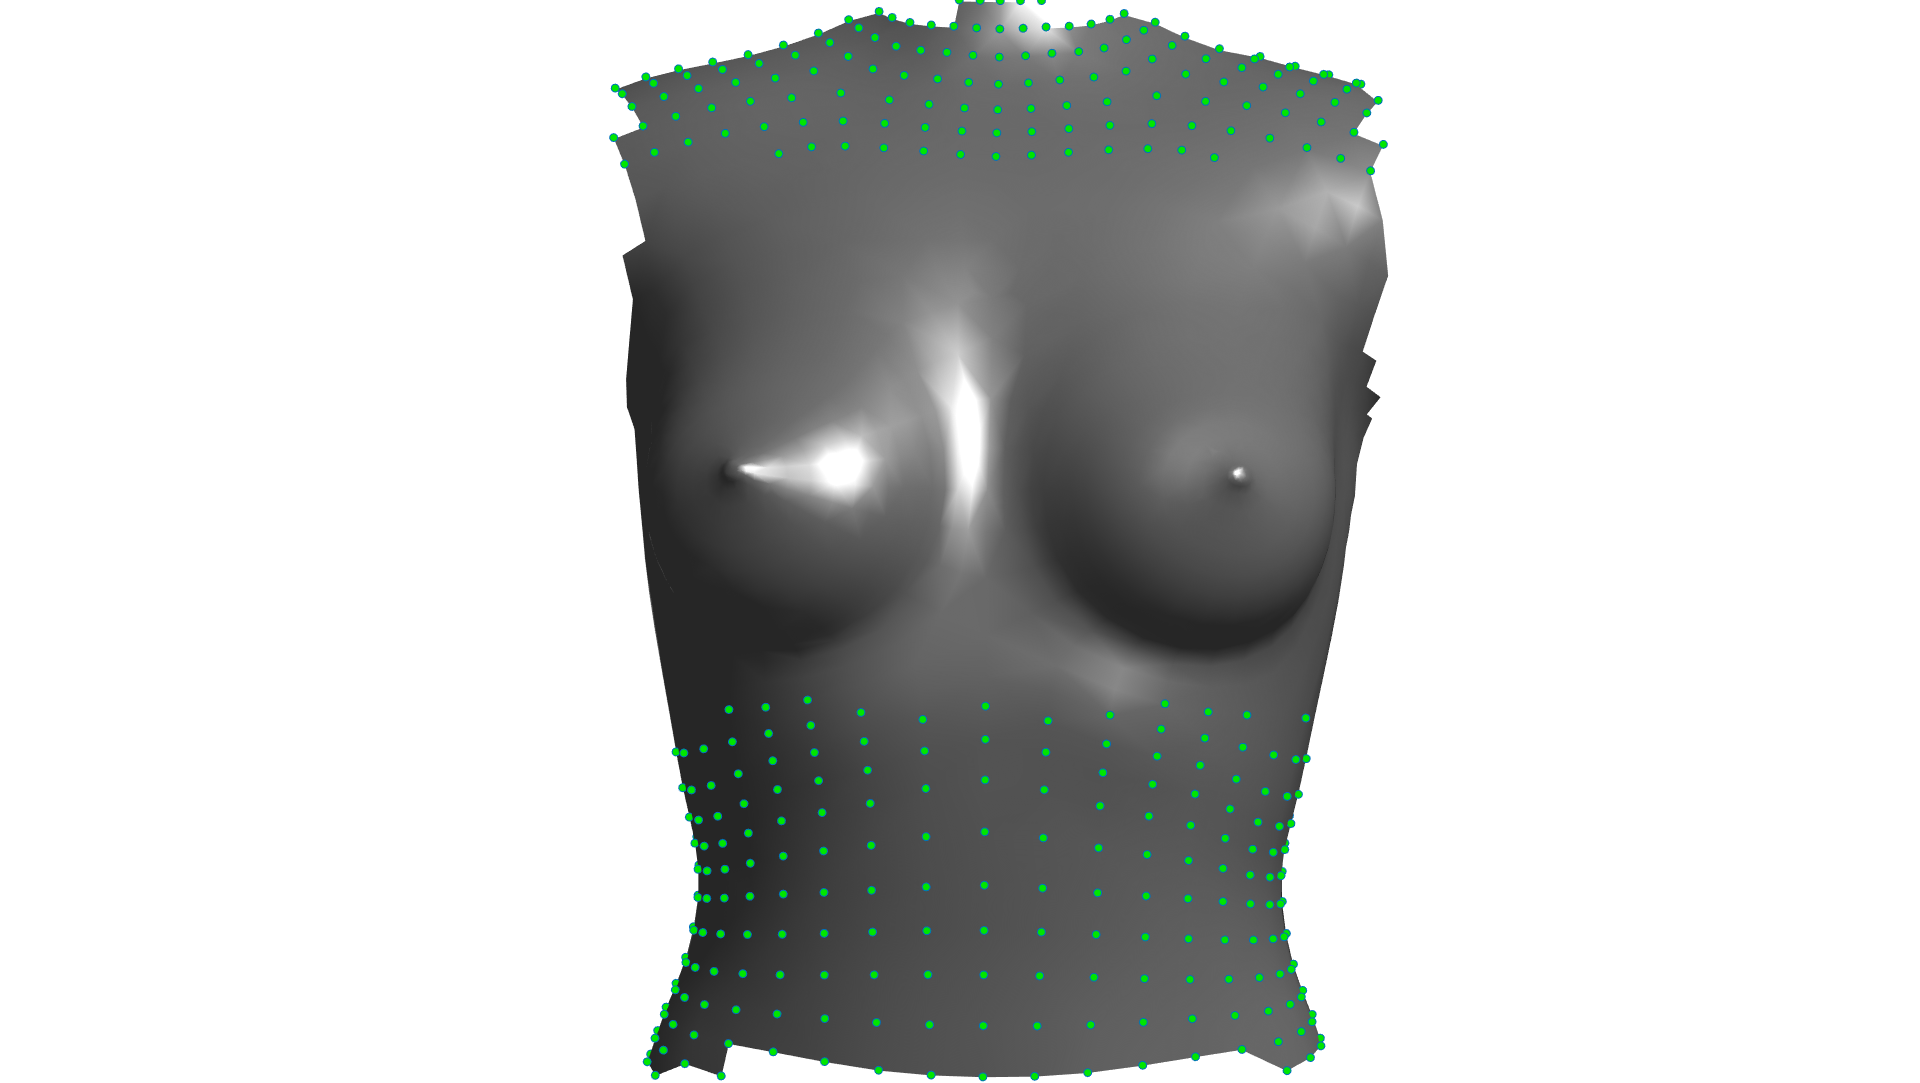
\includegraphics[width=0.75\textwidth]{figures/alignment}
\caption{The mesh is depicted as the grey surface. The points drawn in green are used for the alignment.}
\label{fig:alignment}
\end{figure}

\section{Parametric Model from Meshes}
\label{paramModel}
In this section it is described how a parametric model is obtained using principle component analysis (PCA). Given $n$ meshes $m_i \in \mathbb{R}^{k \times 3}$, where $k$ describes the amound of vertices $m$ has, each mesh needs to be transformed to be of shape $\mathbb{R}^{1 \times 3k}$. Then, all transformed meshes are stacked into a matrix $M \in \mathbb{R}^{n \times 3k}$. As the differences over each column isn't significant, the mean $\bar{m}$ of the matrix $M$ is subtracted from each row of $M$.
\begin{gather}
\mathbf{A} :=
\begin{bmatrix}
 m_1' - \bar{m} \\
 m_2' - \bar{m} \\
 \vdots \\
 m_n' - \bar{m}
\end{bmatrix}
\in \mathbb{R}^{n \times 3k}
\end{gather}

Next, PCA is run with matrix $A$ as the input. PCA is able to reduce the dimensionality of the data while retaining most of the information from the initial data set. This is achieved by finding orthogonal basis vectors, where the first basis vector is responsible for the largest variance in the data. The second basis vector needs to be orthogonal to the first and is responsible for the second largest variance of the data. This holds for each following basis vector. These basis vectors in PCA are also known as principle components.

The output of the PCA function is:

\begin{gather}
\mathbf{coeff} :=
\begin{bmatrix}
 c_1&c_2&\cdots&c_{n-1}
\end{bmatrix}
\in \mathbb{R}^{3k \times n-1}
\end{gather}
\begin{gather}
\mathbf{score} :=
\begin{bmatrix}
s_1&s_2&\cdots&s_{n-1}
\end{bmatrix}
\in \mathbb{R}^{n \times n-1}
\end{gather}

where coefficient $c_i$ is the $i$-th principle component and score $s_i$ is the $i$-th parameter vector corresponding to the $i$-th input. Therefore the input data can be reproduced by computing $\mathbf{A = score \times {coeff}^T}$. Instead of using all $n-1$ coefficients it is possible to only use the first $\mathbf{q}$ coefficients resulting in an approximation of the space. The parameters $\mathbf{p_{q,new}}$ for a new input mesh $m_{new}$ can be easily computed for $\mathbf{q}$ coefficients by first reshaping the mesh to be of the form $\mathbb{R}^{3k \times 1}$ and subtracting the mean $\bar{m}$. This is done the same way as above, adding an additional step to transpose. Then the pseudoinverse of $\mathbf{coeff_{(q)}}$ is multiplied from the left to compute the corresponding parameters $\mathbf{p_{q,new}}$:
\begin{gather}
\mathbf{p_{q,new}} = \mathbf{coeff^+_{(q)}} \cdot (m_{new}' - \bar{m})^T  \text{  where }
\mathbf{coeff_{(q)}} :=
\begin{bmatrix}
 c_1&c_2&\cdots&c_{q}
\end{bmatrix}
\in \mathbb{R}^{3k \times q}
\end{gather}

In this example the parametric model is based on the vertices of the mesh. In the next subsections, two other variants are explored and explained.
\subsection{Face Deformations}
Instead of defining a mesh by its vertices, it is possible to describe it by the deformations of the faces. This is done by defining one source mesh and computing how each face is deformed. One way to quantify a deformation of a face was described by Sumner \cite{sumner2004deformation}, where the idea was to transfer triangle deformations between similar meshes. First, a new vertex needs to be computed such that an affine transformation can be determined. The fourth vertex is defined as follows:
\begin{gather}
  \mathbf{v_4} = \mathbf{v_1} + (\mathbf{v_2} - \mathbf{v_1})\cross(\mathbf{v_3}-\mathbf{v_1})/\sqrt{\lvert(\mathbf{v_2}-\mathbf{v_1})\cross(\mathbf{v_3}-\mathbf{v_1})\rvert} \label{normalequation}
\end{gather}
%% Add image of triangle with a point added along the normal to describe what is happening up here
\begin{figure}[h]
\centering
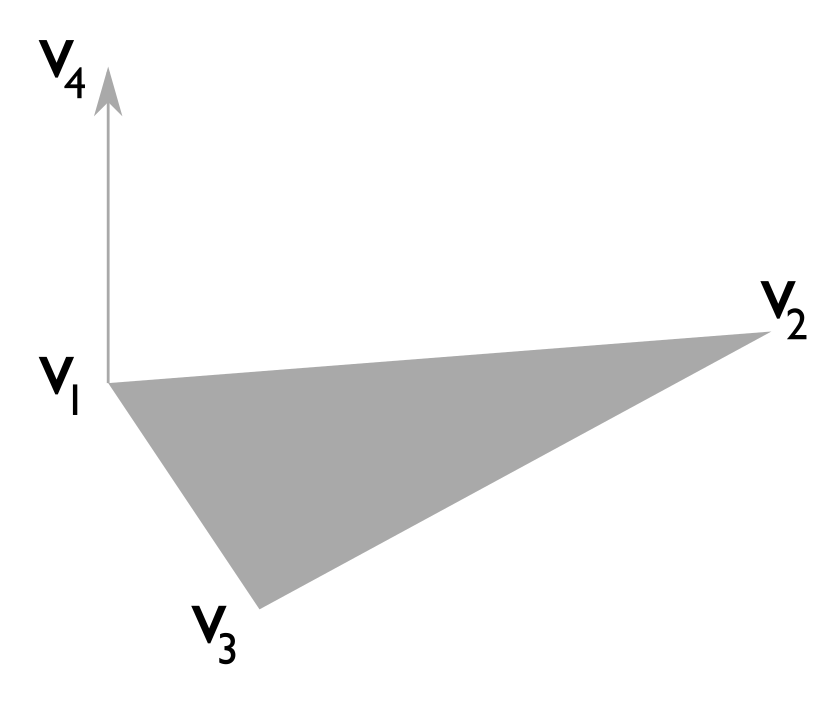
\includegraphics[width=0.25\textwidth]{figures/normal}
\caption{A vertex is added to the triangle that lies in the direction of the normal.}
\label{fig:normal}
\end{figure}

See figure \ref{fig:normal} for a visualization of adding a vertex on the normal.
Given both faces with one additional vertex, the following equations can be posed:
\begin{gather}
 \mathbf{Q}\mathbf{v_i}+\mathbf{d} = \mathbf{\tilde{v}_i}, \mathbf{i} \in \mathbf{1} \dotsc \mathbf{4}
\end{gather}
where $\mathbf{Q} \in \mathbb{R}^{3 \cross 3}$ and translation vector $\mathbf{d}$ describe the affine transformation. By subtracting the first equation from the following three equations and rewriting the resulting system in matrix form, the problem can be defined as $\mathbf{Q}\mathbf{V}=\mathbf{\tilde{V}}$ where
\begin{gather}
  \mathbf{V} =
  \begin{bmatrix}
   \mathbf{v_2} - \mathbf{v_1}&\mathbf{v_2} - \mathbf{v_1}&\mathbf{v_2} - \mathbf{v_1}
  \end{bmatrix} \\
  \mathbf{\tilde{V}} =
  \begin{bmatrix}
   \mathbf{\mathbf{v}_2} - \mathbf{\mathbf{v}_1}&\mathbf{\mathbf{v}_2} - \mathbf{\mathbf{v}_1}&\mathbf{\mathbf{v}_2} - \mathbf{\mathbf{v}_1}
  \end{bmatrix}
\end{gather}
The closed form expression for $\mathbf{Q}$ is defined as
\begin{gather}
  \mathbf{Q}=\mathbf{\tilde{V}}\mathbf{V}^{-1}
\end{gather}
To fully describe a mesh, this $\mathbf{Q}$ matrix needs to be computed for each face of the mesh. Finally, the mesh is represented by $\mathbf{D} \in \mathbb{R}^{3 \times 3h}$ where $\mathbf{h}$ is the number of faces the mesh has. To be able to run PCA, each mesh needs to be reshaped to be of form $\mathbf{D'} \in \mathbb{R}^{1 \times 9h}$ and the rest of the process is the same as above in section \ref{paramModel}.

\subsection{Point Normals}
This method is very much similar to one described in section \ref{paramModel}. In addition to the vertices of the mesh, one vertex per face is computed as described in equation \ref{normalequation} and added to the list of vertices of the mesh. Therefore the mesh matrix will be of form $\mathbb{R}^{k+h \times 3}$ where $\mathbf{k}$ is the number of original vertices and $\mathbf{h}$ is the number of faces of the mesh.

\section{Mapping}
The following segment describes how a mapping can be computed in a linear or a non-linear way. The data available is the parameters returned from the both parametric models for the before and after examples. The matrices of the data are
\begin{gather}
  \mathbf{P_{before}} =
  \begin{bmatrix}
    \mathbf{p_{b,1}} \\
    \mathbf{p_{b,2}}  \\
    \vdots \\
    \mathbf{p_{b,n}}
  \end{bmatrix}
  \in \mathbb{R}^{n \cross n-1},
  \mathbf{P_{after}} =
  \begin{bmatrix}
    \mathbf{p_{a,1}} \\
    \mathbf{p_{a,2}} \\
    \vdots \\
    \mathbf{p_{a,n}}
  \end{bmatrix}
  \in \mathbb{R}^{n \cross n-1}
\end{gather}
where each parameter pair $(\mathbf{p_{b,i}}, \mathbf{p_{a,i}})\ \forall i$ is related, as the after was generated from the before.

\subsection{Linear Method}
The first method used, was the linear system solver by MATLAB (also known as backslash \ solver) that solved the equation
\begin{gather}
  \mathbf{P_{before}} \cdot \mathbf{M_{linear}} = \mathbf{P_{after}}
  \text{where} M_{linear} \in \mathbb{R}^{n-1 \times n-1}.
\end{gather}
It is clear that an explicit linear transformation could be found for each parameter pair, but the goal is to have one mapping that works for each parameter pair.
\subsection{Non-Linear Variants}
These next few methods are all part of the python scikit-learn library \cite{scikit-learn}.
\subsubsection{Random Forest}

\subsubsection{Decision Tree}

\subsubsection{Multilayer Perceptron}

\section{Parametric Model from Editor}

\section{Evaluation}

\subsection{Mapping Error}
% Compare to GT

\subsection{Fit to Pointcloud}
% Compare to NRICP+SimonResultCeres
